% ============================================================================
% MQFS Working Paper (unnumbered)
% Pricing Satellite-Indexed Parametric Crop-Insurance Derivatives over Sicily
% (c) Nicolo Angileri / Mediterranean Quantitative Finance Society. MIT Licence.
% Compile:  pdflatex mqfs_wp_satellite_crop.tex   (run twice for references)
% ============================================================================
\documentclass[11pt]{article}

\usepackage[a4paper,margin=2.4cm]{geometry}
\usepackage{amsmath,amssymb}
\usepackage{booktabs}
\usepackage{graphicx}
\usepackage{xcolor}
\usepackage[most]{tcolorbox}
\usepackage{listings}
\usepackage{fancyhdr}
\usepackage{titlesec}
\usepackage[hidelinks]{hyperref}
\usepackage{caption}
\usepackage{enumitem}

\graphicspath{{../figures/}{figures/}}
% Auto-generated by scripts/run_pipeline.py — do not edit by hand.
\newcommand{\resFair}{2\,019.30}
\newcommand{\resSD}{3\,302.61}
\newcommand{\resWang}{2\,596.87}
\newcommand{\resTrigger}{22.6}
\newcommand{\resCVaR}{20\,523.54}
\newcommand{\resVaR}{13\,967.21}
\newcommand{\resEIfTrig}{9\,053.55}
\newcommand{\ouKappa}{1.91}
\newcommand{\ouSigma}{0.248}
\newcommand{\ouHalfLife}{0.36}
\newcommand{\contractStrike}{0.452}
\newcommand{\contractTick}{250\,000.00}
\newcommand{\contractLimit}{50\,000.00}
\newcommand{\mcPaths}{200\,000}
\newcommand{\nSeasons}{11}
\newcommand{\nEpisodes}{7}
\newcommand{\riskWindow}{75--151}
\newcommand{\nDekads}{8}
\newcommand{\mktR}{3.0}
\newcommand{\mktTheta}{0.25}
\newcommand{\mktLambda}{0.15}


% --- palette ---------------------------------------------------------------
\definecolor{mqfsnavy}{HTML}{1B3A66}
\definecolor{mqfsblue}{HTML}{2F6DB0}
\definecolor{mqfsgrey}{HTML}{5B6470}
\definecolor{mqfslight}{HTML}{EEF3F8}

\hypersetup{colorlinks=true, linkcolor=mqfsnavy, urlcolor=mqfsblue, citecolor=mqfsnavy}

% --- section styling -------------------------------------------------------
\titleformat{\section}{\large\bfseries\color{mqfsnavy}}{\thesection}{0.7em}{}
\titleformat{\subsection}{\normalsize\bfseries\color{mqfsnavy}}{\thesubsection}{0.6em}{}
\captionsetup{font=small,labelfont={bf,color=mqfsnavy}}

% --- header / footer -------------------------------------------------------
\pagestyle{fancy}
\fancyhf{}
\lhead{\footnotesize\color{mqfsgrey}MQFS Working Paper}
\rhead{\footnotesize\color{mqfsgrey}Satellite-Indexed Parametric Crop Insurance}
\lfoot{\footnotesize\color{mqfsgrey}\textcopyright\ Nicol\`o Angileri. MIT Licence.}
\rfoot{\footnotesize\color{mqfsgrey}\thepage}
\renewcommand{\headrulewidth}{0.4pt}
\renewcommand{\footrulewidth}{0.4pt}

% --- callout box -----------------------------------------------------------
\newtcolorbox{keybox}[1][]{
  colback=mqfslight, colframe=mqfsnavy, boxrule=0.6pt, arc=2pt,
  left=8pt, right=8pt, top=6pt, bottom=6pt, fonttitle=\bfseries, #1}

\lstset{
  basicstyle=\ttfamily\scriptsize, breaklines=true,
  backgroundcolor=\color{mqfslight}, frame=single, rulecolor=\color{mqfsgrey},
  numbers=none, columns=fullflexible, keepspaces=true}

\setlength{\parindent}{0pt}
\setlength{\parskip}{0.55em}

% ============================================================================
\begin{document}

% ---------------------------------------------------------------- title block
\begin{center}
  {\footnotesize\color{mqfsgrey}\textsc{Mediterranean Quantitative Finance Society} \quad$\cdot$\quad Working Paper}\\[0.4em]
  {\LARGE\bfseries\color{mqfsnavy} Pricing Satellite-Indexed Parametric\\[0.15em]
   Crop-Insurance Derivatives over Sicily}\\[0.7em]
  {\large An end-to-end pipeline from Sentinel-2 vegetation indices to a multi-language Monte~Carlo pricer}\\[1.0em]
  {\normalsize\bfseries Nicol\`o Angileri}\\[0.2em]
  {\footnotesize Mediterranean Quantitative Finance Society (MQFS)}\\[0.2em]
  {\footnotesize\color{mqfsgrey}\today}
\end{center}
\vspace{0.4em}
\hrule height 0.8pt
\vspace{0.9em}

% ------------------------------------------------------------------- abstract
\begin{abstract}
\noindent
We design and implement a complete, reproducible pipeline for pricing
\emph{parametric} crop-insurance derivatives whose settlement index is built
directly from satellite imagery rather than from ground weather stations. The
underlying is a seasonal vegetation index --- the dekadal mean NDVI of a Sicilian
durum-wheat belt over the grain-filling window --- derived from Sentinel-2
surface reflectance. Because a vegetation index is not a traded asset, the
market is incomplete and textbook risk-neutral replication does not apply; we
price instead with two transparent incomplete-market principles, the actuarial
standard-deviation loading and the Wang (2000) distortion, both of which collapse
to the discounted burn cost in the no-load limit. NDVI dynamics are modelled as a
deterministic harmonic climatology plus a mean-reverting Ornstein--Uhlenbeck
anomaly, calibrated in closed form on the de-seasonalised residual. The Monte
Carlo engine is implemented four times --- in NumPy, portable C, OpenMP-parallel
C\texttt{++}, and MATLAB --- with the three numerical engines agreeing to within
Monte Carlo standard error, a deliberate audit control. On a synthetic but
realistic ten-season calibration the reference contract prices at a fair (burn)
value of EUR~\resFair{}, an SD-principle premium of EUR~\resSD{}, and a Wang
premium of EUR~\resWang{}, with a trigger probability of \resTrigger\%. All code,
tests, and this paper are open source under the MIT licence.
\end{abstract}

\smallskip
{\footnotesize\textbf{Keywords:} parametric insurance; weather derivatives;
NDVI; remote sensing; incomplete markets; Wang transform; Ornstein--Uhlenbeck;
Monte Carlo; Sicily; durum wheat.\par
\textbf{JEL:} G13, G22, Q14, C63, C53.}

\vspace{0.6em}
\hrule height 0.4pt
\vspace{0.4em}

% =============================================================== 1 Introduction
\section{Introduction}
Mediterranean agriculture is acutely exposed to drought, and Sicilian durum
wheat --- the backbone of the island's cereal economy and of national pasta
supply chains --- is no exception. Traditional indemnity insurance against such
losses is slow and costly to administer: each claim requires an on-site loss
adjuster, and asymmetric information invites moral hazard and adverse selection.
\emph{Parametric} insurance sidesteps this by paying out on an objective,
independently measurable index rather than on assessed loss. The contract here
pays the grower when a satellite-measured vegetation index over the growing
season falls below a contractual strike.

The premise of this paper is that the settlement index can be sourced entirely
from space. The European Copernicus programme distributes Sentinel-2 surface
reflectance at 10--20\,m resolution with a revisit of a few days and a free,
open licence. From it we compute the Normalised Difference Vegetation Index
(NDVI), a decades-old proxy for canopy greenness and photosynthetic activity
that correlates strongly with end-of-season cereal yield. Pricing a derivative
on this index requires three things done carefully: a disciplined geospatial
ingestion layer, a statistical model that respects the bounded, seasonal,
mean-reverting nature of NDVI, and a pricing methodology honest about the fact
that the underlying cannot be hedged.

\begin{keybox}[title=Contribution]
We deliver (i) a config-driven, offline-reproducible pipeline from Sentinel-2
ingestion to a priced contract; (ii) an incomplete-market pricing treatment with
two defensible premium principles; (iii) a seasonal-mean~+~OU model calibrated in
closed form; and (iv) a four-language implementation (NumPy / C / C\texttt{++} /
MATLAB) whose three numerical engines are cross-validated to Monte Carlo standard
error. Everything is open source.
\end{keybox}

This paper follows the structure of earlier MQFS work on Mediterranean risk: we
describe the data and pipeline (\S2), the signal (\S3), the pricing model (\S4),
the calibration and results (\S5), the Sicilian application (\S6), and the
multi-language software architecture (\S7) before concluding (\S8).

% ====================================================== 2 Data and the pipeline
\section{Data and the Geospatial Pipeline (``The Oracle'')}
\subsection{Sensor and area of interest}
The area of interest is the island of Sicily, with three illustrative pricing
zones isolated for basis-risk diversification: a durum-wheat belt
(Caltanissetta--Enna), the Catania citrus plain, and the Trapani
vineyard/olive district. The sensor is Sentinel-2 L2A surface reflectance
(\texttt{COPERNICUS/S2\_SR\_HARMONIZED}) over 2016--2026. Pixels are restricted to
cropland using the ESA WorldCover layer, so that urban, forest and water pixels
do not contaminate the agricultural signal.

\subsection{From raw scenes to a clean index}
Two ingestion paths are provided. The first runs server-side on Google Earth
Engine, masking cloud and shadow with the Scene Classification Layer and reducing
to 10-day (dekadal) median composites entirely in the cloud, so that only a
compact time series is ever downloaded. The second is a local, memory-disciplined
path over Copernicus tiles using lazy, chunked \texttt{rioxarray}/Dask reads,
deterministic file-handle release, and \texttt{float32} throughout. Dekadal
median compositing is the operational standard for phenology: it is robust to
residual cloud and to bidirectional reflectance effects, and it regularises the
irregular revisit cadence onto a fixed grid.

\begin{keybox}[title=NDVI and the water indices]
NDVI${}=(\rho_{\text{NIR}}-\rho_{\text{red}})/(\rho_{\text{NIR}}+\rho_{\text{red}})$
measures greenness. We distinguish it carefully from the two ``NDWI'' indices that
are routinely conflated: the McFeeters NDWI (green/NIR) detects \emph{open water},
whereas the Gao index NDMI${}=(\rho_{\text{NIR}}-\rho_{\text{SWIR}})/(\rho_{\text{NIR}}+\rho_{\text{SWIR}})$
tracks canopy \emph{moisture stress}. For drought monitoring it is the moisture
index, not the open-water one, that matters; both are implemented.
\end{keybox}

% ============================================== 3 Feature engineering / signal
\section{Feature Engineering and the Yield-Shock Signal (``The Quant Layer'')}
The raw composite series is gap-filled and denoised with a Whittaker smoother,
which penalises roughness while honouring the data and interpolates across
cloud-induced gaps. We then fit a day-of-year \emph{climatology} by harmonic
regression (two Fourier orders): this is the deterministic seasonal mean
$s(\text{doy})$ that a healthy crop tracks in an average year.

The \emph{anomaly} is the de-seasonalised residual, standardised to a $z$-score.
A complementary, scale-free indicator is the Vegetation Condition Index
$\text{VCI}=(\text{NDVI}-\text{NDVI}_{\min})/(\text{NDVI}_{\max}-\text{NDVI}_{\min})$,
computed per composite period so that 0 marks the worst and 1 the best greenness
on record for that point in the season. A \emph{yield shock} --- the event the
insurance is written against --- is flagged when the $z$-score drops below
$-1.5$ or VCI below $0.35$; consecutive flagged dekads are grouped into drought
episodes with a depth and duration.

\begin{figure}[h]
\centering
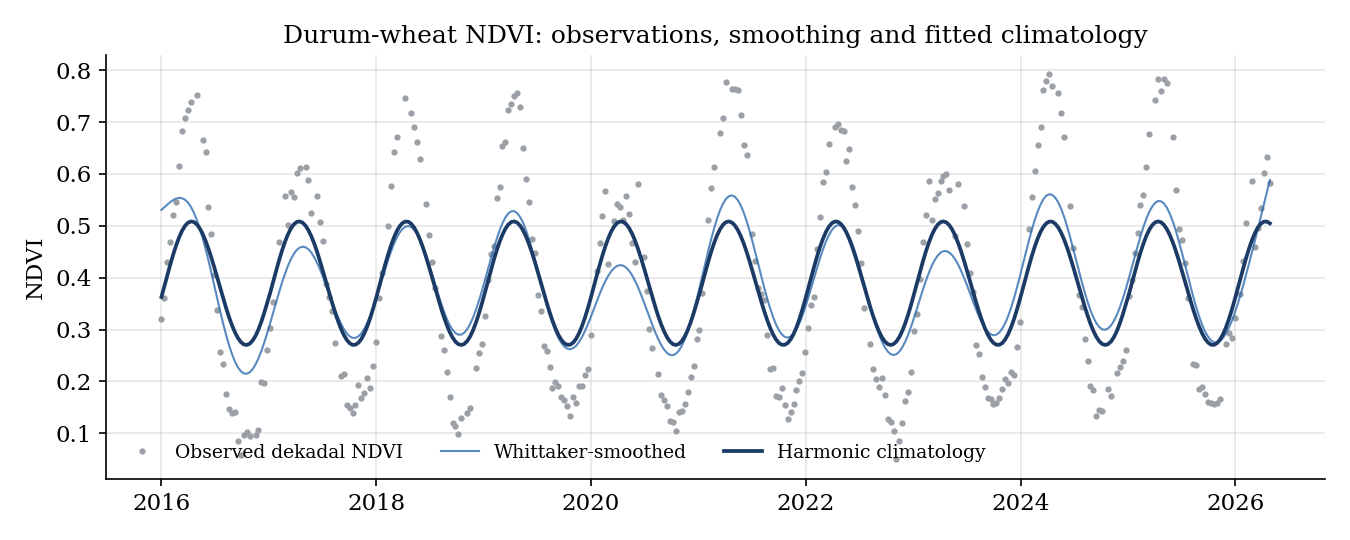
\includegraphics[width=0.95\textwidth]{fig_ndvi_climatology.png}
\caption{Dekadal NDVI for the durum-wheat zone with the Whittaker-smoothed series
and the fitted harmonic climatology. The climatology captures the
autumn-emergence, spring-peak, summer-senescence cycle of a Mediterranean winter
cereal.}
\label{fig:clim}
\end{figure}

\begin{figure}[h]
\centering
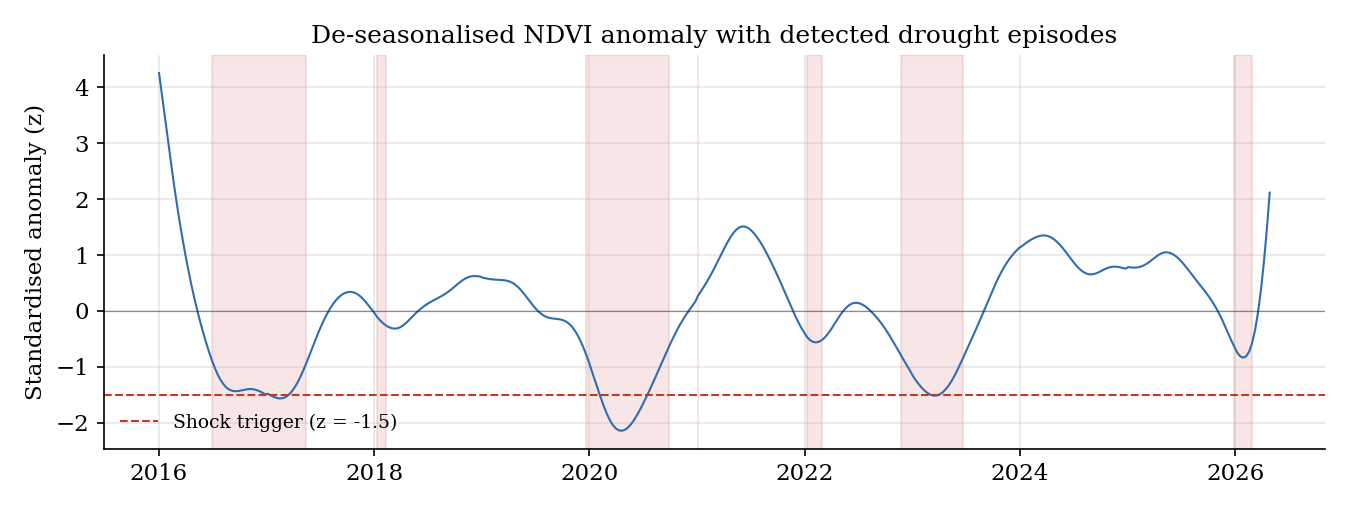
\includegraphics[width=0.95\textwidth]{fig_anomaly_episodes.png}
\caption{De-seasonalised NDVI anomaly ($z$-score). Shaded spans are detected
drought episodes; the pipeline recovers \nEpisodes\ episodes over the sample,
with the deepest troughs aligning with the injected drought seasons.}
\label{fig:anom}
\end{figure}

% =================================================== 4 Pricing model
\section{The Pricing Model: an Incomplete-Market Argument}
\subsection{Why not risk-neutral replication}
A vegetation index is \textbf{not a traded asset}. There is no self-financing
portfolio in ``satellite greenness'', so the market is incomplete and there is no
unique equivalent martingale measure obtained by replication. Pricing a crop
derivative by naive risk-neutral expectation is therefore a category error. The
two routes we take are standard in the actuarial and weather-derivative
literature.

\subsection{Premium principles}
Let $Y$ be the contract payout and $r,T$ the risk-free rate and tenor. The
\emph{fair (burn) value} is the discounted expected payout,
$\Pi_0=e^{-rT}\,\mathbb{E}_{\mathbb P}[Y]$. The \emph{standard-deviation
principle} adds a transparent loading proportional to risk,
\begin{equation}
\Pi_{\text{SD}}=e^{-rT}\bigl(\mathbb{E}_{\mathbb P}[Y]+\theta\,\mathrm{SD}_{\mathbb P}[Y]\bigr).
\end{equation}
The \emph{Wang transform} (Wang, 2000) distorts the survival function of the loss
by the market price of risk $\lambda$,
\begin{equation}
\Pi_{\text{Wang}}=e^{-rT}\!\int_0^{\infty} g\!\left(\widehat S_Y(y)\right)\,dy,
\qquad g(u)=\Phi\!\left(\Phi^{-1}(u)+\lambda\right),
\end{equation}
which loads the adverse tail and is consistent with CAPM/Black--Scholes in the
Gaussian traded limit. Both reduce to $\Pi_0$ when $\theta=\lambda=0$.

\subsection{NDVI dynamics}
NDVI is bounded, seasonal and mean-reverting, so geometric Brownian motion is
inappropriate. We model the in-season index as the climatology plus a
mean-reverting Ornstein--Uhlenbeck anomaly. Discretised at a dekadal step
$\Delta t$ (in years), for $k=1,\dots,M$,
\begin{equation}
X_k=a\,X_{k-1}+b\,Z_k,\quad
a=e^{-\kappa\Delta t},\;
b=\sigma\sqrt{\tfrac{1-e^{-2\kappa\Delta t}}{2\kappa}},\;
Z_k\sim\mathcal N(0,1),
\end{equation}
\begin{equation}
\text{NDVI}_k=\mathrm{clip}\bigl(s_k+X_k,\,\text{floor},\,\text{cap}\bigr),\qquad
I=\tfrac1M\textstyle\sum_k \text{NDVI}_k .
\end{equation}
The settlement index $I$ is the seasonal mean (integral and minimum variants are
also supported). The put-style payout, with tick $c$, strike $K$ and limit $L$, is
$Y=\min\!\bigl(L,\,c\,\max(0,K-I)\bigr)$.

\begin{keybox}[title=Calibration discipline]
The OU driver is calibrated on the \emph{raw} de-seasonalised residual, not on
the smoothed series. Smoothing is the right tool for signal extraction and VCI,
but calibrating the stochastic term on it removes the very variance the term must
reproduce and collapses the model-implied trigger probability to zero. Calibrating
on the raw residual recovers a seasonal-index dispersion consistent with the
historical record and with the percentile strike.
\end{keybox}

As an internal check, the Monte Carlo expected shortfall is compared against the
closed-form Bachelier (Gaussian) put on the index,
$\mathbb E[\max(0,K-I)]=(K-m)\Phi(\tfrac{K-m}{\varsigma})+\varsigma\,\phi(\tfrac{K-m}{\varsigma})$
for $I\sim\mathcal N(m,\varsigma)$; the two agree within sampling error in the test
suite.

% ====================================================== 5 Calibration & results
\section{Calibration and Results}
The contract is calibrated on \nSeasons\ seasons of the durum-wheat zone over the
grain-filling risk window (day-of-year \riskWindow, $M=\nDekads$ dekads). The
strike is set data-free at the 20th percentile of the historical seasonal index,
$K=\contractStrike$. The OU fit gives $\kappa=\ouKappa$ (half-life $\ouHalfLife$
years) and $\sigma=\ouSigma$. Market parameters are $r=\mktR\%$, $\theta=\mktTheta$
and $\lambda=\mktLambda$, with \mcPaths\ antithetic Monte Carlo paths.

\begin{table}[h]
\centering
\caption{Pricing sheet for the reference durum-wheat drought put. Tick
EUR~\contractTick\ per NDVI unit, payout cap (limit) EUR~\contractLimit.}
\label{tab:pricing}
\begin{tabular}{lr}
\toprule
Quantity & Value (EUR) \\
\midrule
Fair (burn) value & 2\,019.30 \\
SD-principle premium & 3\,302.61 \\
Wang-transform premium & 2\,596.87 \\
Expected payout (undiscounted) & 2\,049.82 \\
Trigger probability & 22.6\% \\
$\mathbb{E}[\text{payout}\mid\text{triggered}]$ & 9\,053.55 \\
Writer VaR 95\% & 13\,967.21 \\
Writer CVaR 95\% & 20\,523.54 \\
\bottomrule
\end{tabular}

\end{table}

The premium ordering is the expected one: the Wang premium (EUR~\resWang)
sits above the fair value (EUR~\resFair) and below the SD-principle premium
(EUR~\resSD) at these loadings. The trigger probability of \resTrigger\% is
consistent with a strike placed at the 20th historical percentile. The writer's
95\% conditional VaR is EUR~\resCVaR, the relevant figure for capital and
reinsurance.

\begin{figure}[h]
\centering
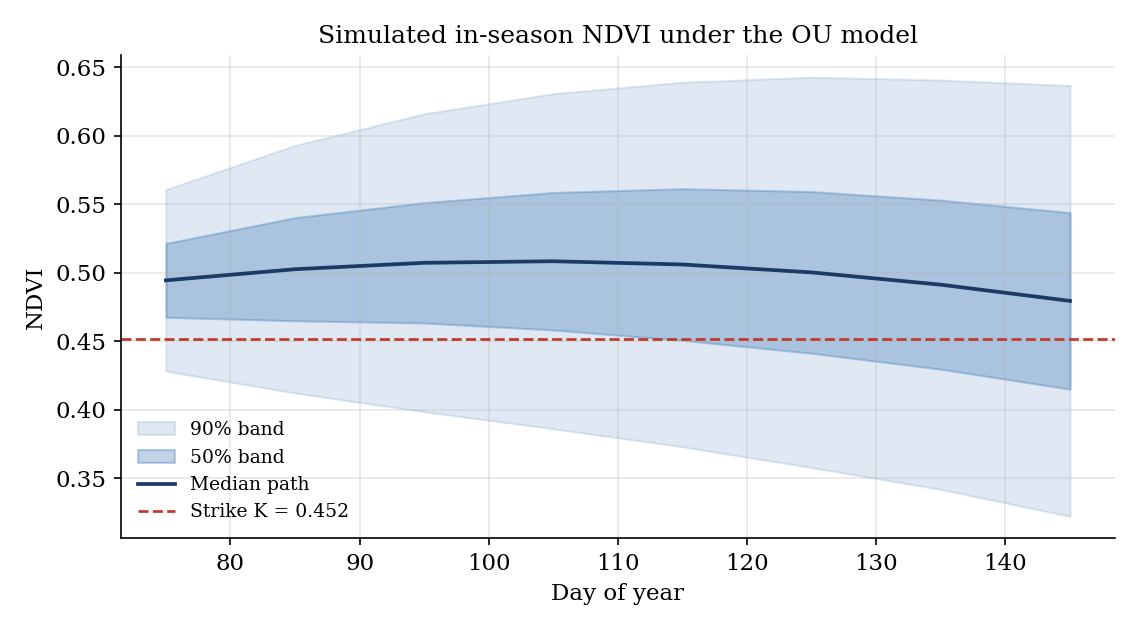
\includegraphics[width=0.78\textwidth]{fig_fan_chart.png}
\caption{Simulated in-season NDVI under the calibrated OU model: median path with
50\% and 90\% bands, and the contractual strike. The strike is placed on the
\emph{seasonal-mean} settlement index $I$; since $I$ averages the path, its
dispersion is tighter than that of the individual dekads shown here. The contract
pays when the realised seasonal index lands below the strike line.}
\label{fig:fan}
\end{figure}

\begin{figure}[h]
\centering
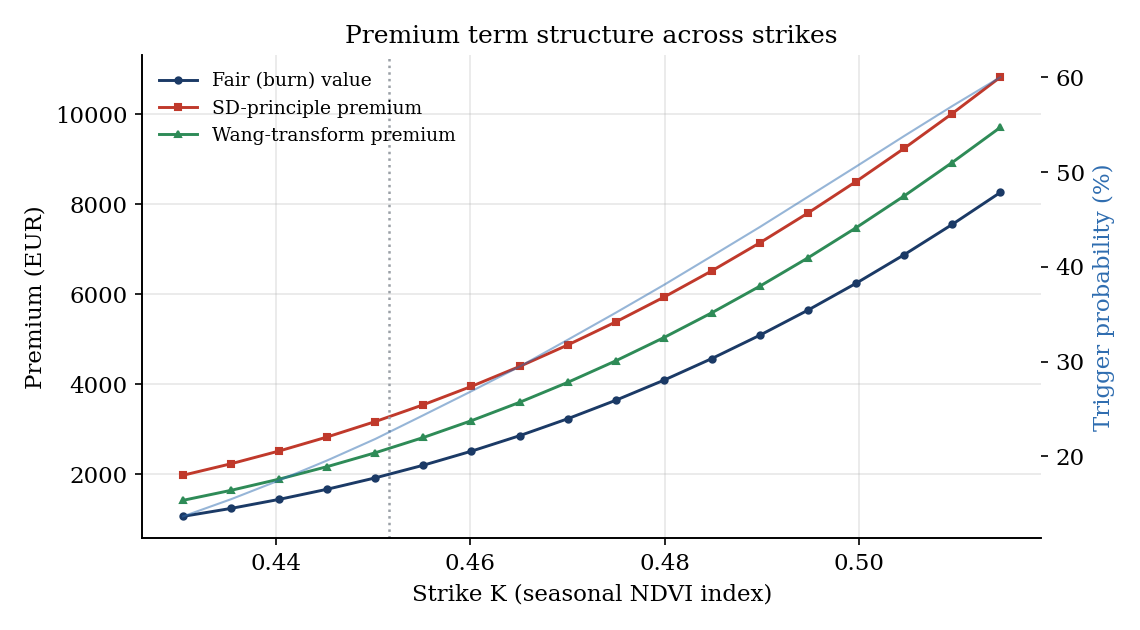
\includegraphics[width=0.82\textwidth]{fig_premium_vs_strike.png}
\caption{Premium term structure across strikes for the three principles, with the
trigger probability (right axis). Premiums rise monotonically with the protection
level; the dotted line marks the reference strike.}
\label{fig:strikes}
\end{figure}

\begin{figure}[h]
\centering
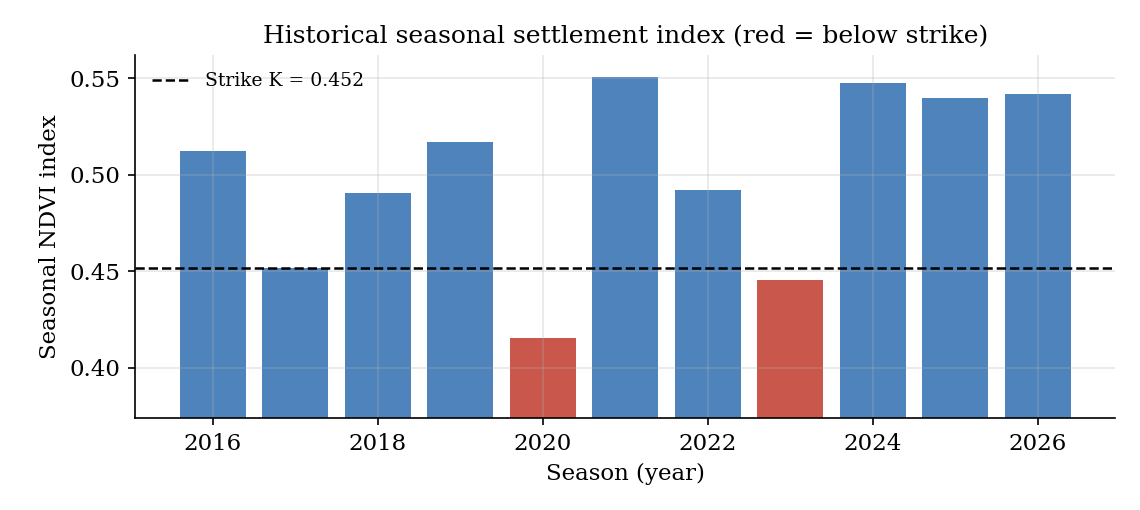
\includegraphics[width=0.82\textwidth]{fig_seasonal_index.png}
\caption{Historical seasonal settlement index by season. Bars below the strike
(red) are the seasons in which the contract would have paid out --- the model-free
burn-cost view that anchors the priced premium.}
\label{fig:seasidx}
\end{figure}

\subsection{Engine cross-validation}
The same contract is priced by the NumPy reference, the C kernel and the
C\texttt{++} engine. The three agree to within Monte Carlo standard error
(Table~\ref{tab:val}, Figure~\ref{fig:val}) --- three independent
implementations, with different random-number generators, converging on the same
priced quantities. This is the central correctness control of the project.

\begin{table}[h]
\centering
\caption{Engine cross-validation. The three implementations agree within Monte
Carlo standard error on every priced quantity.}
\label{tab:val}
\begin{tabular}{lrrrr}
\toprule
Engine & Fair value & SD premium & Trigger (\%) & CVaR 95\% \\
\midrule
NumPy & 2\,019.30 & 3\,302.61 & 22.64 & 20\,523.54 \\
C & 2\,002.55 & 3\,277.47 & 22.55 & 20\,387.28 \\
C++ & 2\,023.58 & 3\,311.19 & 22.58 & 20\,615.07 \\
\midrule
MC standard error & \multicolumn{4}{l}{$11.48$ on the fair value (discounted mean payout)} \\
\bottomrule
\end{tabular}

\end{table}

\begin{figure}[h]
\centering
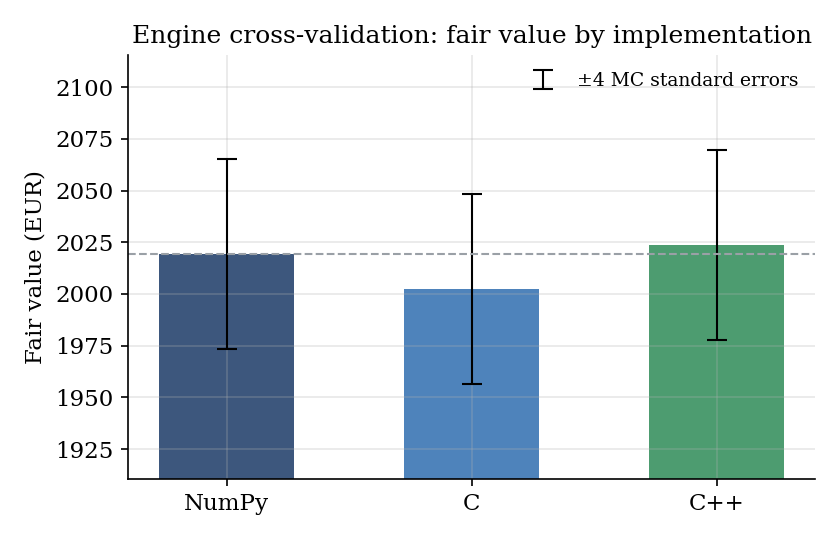
\includegraphics[width=0.62\textwidth]{fig_engine_validation.png}
\caption{Fair value by implementation with $\pm4$ Monte Carlo standard-error
bars. The spread between engines is a small fraction of the sampling error.}
\label{fig:val}
\end{figure}

\begin{figure}[h]
\centering
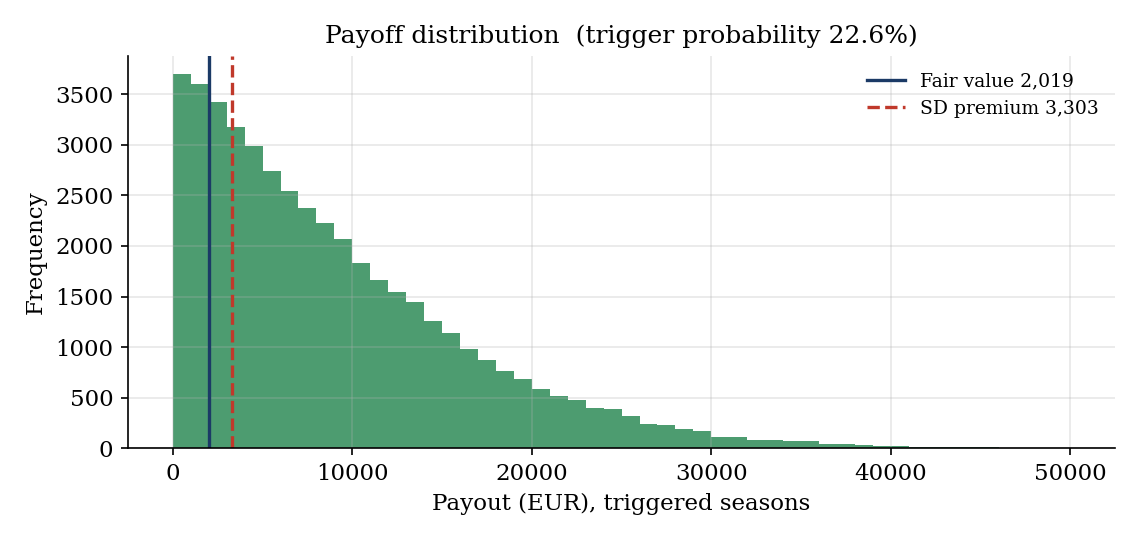
\includegraphics[width=0.82\textwidth]{fig_payoff_distribution.png}
\caption{Distribution of payouts on triggered paths, with the fair value and the
SD-principle premium marked. The long right tail --- capped at the contractual
limit --- is what the risk loading and the Wang distortion price.}
\label{fig:payoff}
\end{figure}

% ======================================================= 6 Sicilian application
\section{Sicilian Application}
The three zones illustrate how the same machinery serves different Sicilian
agricultural sectors and how multi-zone contracts diversify basis risk --- the
residual mismatch between the satellite index and an individual grower's realised
loss. For durum wheat the grain-filling window (mid-March to end-May) is decisive:
heat and water stress in this phase truncate grain weight and therefore yield, and
it is exactly this window the contract insures. Citrus and vineyard zones have
different phenological windows and stress signatures, which the same climatology
machinery accommodates by re-fitting per zone. Because Sentinel-2 is free and
global, the approach extends directly to other Mediterranean cereal regions
without new ground infrastructure.

\begin{keybox}[title=Basis risk]
Parametric payouts depend on the index, not on the individual farm, so a grower
can suffer a loss the index does not register, or vice versa. Tightening the
spatial mask to cropland, pricing zones separately, and choosing the risk window
to match the crop's critical phase all reduce --- but cannot eliminate --- this
basis risk. It is the principal limitation of any index insurance and is stated
plainly to the insured.
\end{keybox}

% ============================================== 7 Implementation architecture
\section{Multi-Language Implementation Architecture}
The system is deliberately polyglot, with each language used where it is
strongest and a single shared model specification across all four.

\begin{itemize}[leftmargin=1.4em,itemsep=2pt]
\item \textbf{Python} orchestrates: geospatial ingestion, feature engineering,
calibration, and the reference NumPy Monte Carlo that defines the numerics.
\item \textbf{C} provides a zero-dependency ``audit kernel'' (xoshiro256\texttt{**}
RNG, Box--Muller normals, \texttt{qsort} tail risk) callable from Python via
\texttt{ctypes} or from MATLAB via \texttt{loadlibrary} --- small enough to read in
one sitting.
\item \textbf{C\texttt{++}} is the production engine: header-only, C\texttt{++}17,
OpenMP-parallel with per-thread generators and antithetic variates, templated on
the payoff functor, exposing the identical C ABI plus an optional pybind11 module.
\item \textbf{MATLAB} mirrors the calibration, pricing, Wang transform and
burn-cost backtest, and produces research figures.
\end{itemize}

The C and C\texttt{++} engines share the exact C ABI of the audit header, which is
how ABI identity --- and therefore numerical comparability --- is guaranteed. A
28-test \texttt{pytest} suite covers the indices, the calibration round-trip, the
economic invariants of the premium, the Bachelier check, and the NumPy-vs-C and
NumPy-vs-C\texttt{++} agreement.

\begin{lstlisting}[caption={Pricing one contract through the reference engine.},captionpos=b]
from pricing_engine.pricer import MarketParams, price_contract
res = price_contract(seasonal, kappa, sigma, dt, contract, MarketParams())
print(res.pretty())            # fair value, SD & Wang premiums, VaR / CVaR
\end{lstlisting}

\begin{keybox}[title=Reproducibility]
Every figure and every number in this paper, including the pricing and validation
tables, is produced by a single command, \texttt{python scripts/run\_pipeline.py},
under a fixed random seed. The tables are generated as \LaTeX{} and included
directly; no value is transcribed by hand. The synthetic calibration runs fully
offline, and live Sentinel-2 archives plug in through the same ingestion layer
without changing the downstream model.
\end{keybox}

% ======================================================= 8 Conclusion
\section{Conclusion}
We have shown that a parametric crop-insurance derivative can be priced
end-to-end from open satellite imagery with institutional rigour: a disciplined
geospatial pipeline, a model faithful to the bounded and seasonal nature of
vegetation indices, an incomplete-market pricing treatment that does not pretend
the underlying is hedgeable, and a multi-language implementation cross-validated
to Monte Carlo standard error. The figures and the pricing sheet in this paper are
generated by running the code, not by hand. The natural extensions are to
calibrate on live Sentinel-2 archives via the provided ingestion layer, to fit
zone-specific yield--index regressions that quantify basis risk explicitly, and to
extend the anomaly model with heavier tails for extreme drought.

% ======================================================= References
\section*{References}
{\small
\begin{itemize}[leftmargin=1.2em,itemsep=1pt,label={}]
\item Wang, S.~S. (2000). A class of distortion operators for pricing financial
and insurance risks. \emph{Journal of Risk and Insurance}, 67(1), 15--36.
\item Kogan, F.~N. (1995). Application of vegetation index and brightness
temperature for drought detection. \emph{Advances in Space Research}, 15(11),
91--100.
\item Gao, B.-C. (1996). NDWI --- a normalized difference water index for remote
sensing of vegetation liquid water from space. \emph{Remote Sensing of
Environment}, 58(3), 257--266.
\item McFeeters, S.~K. (1996). The use of the Normalized Difference Water Index
(NDWI) in the delineation of open water features. \emph{International Journal of
Remote Sensing}, 17(7), 1425--1432.
\item Eilers, P.~H.~C. (2003). A perfect smoother. \emph{Analytical Chemistry},
75(14), 3631--3636.
\item Vasicek, O. (1977). An equilibrium characterization of the term structure.
\emph{Journal of Financial Economics}, 5(2), 177--188.
\item Jewson, S., \& Brix, A. (2005). \emph{Weather Derivatives Valuation}.
Cambridge University Press.
\item Drusch, M., et al. (2012). Sentinel-2: ESA's optical high-resolution mission
for GMES operational services. \emph{Remote Sensing of Environment}, 120, 25--36.
\end{itemize}}

\vfill
\begin{center}\footnotesize\color{mqfsgrey}\rule{0.5\textwidth}{0.4pt}\\[0.4em]
\textcopyright\ Nicol\`o Angileri. Released under the MIT Licence.\\
The Mediterranean Quantitative Finance Society (MQFS) is an independent student
research initiative and is not affiliated with the University of Palermo.
\end{center}

\end{document}
